% pred-review.tex

\documentclass[tikz, border=2pt]{standalone}

\usepackage[dvipsnames]{xcolor}
\usetikzlibrary{arrows.meta, positioning, shapes.geometric}

\begin{document}
  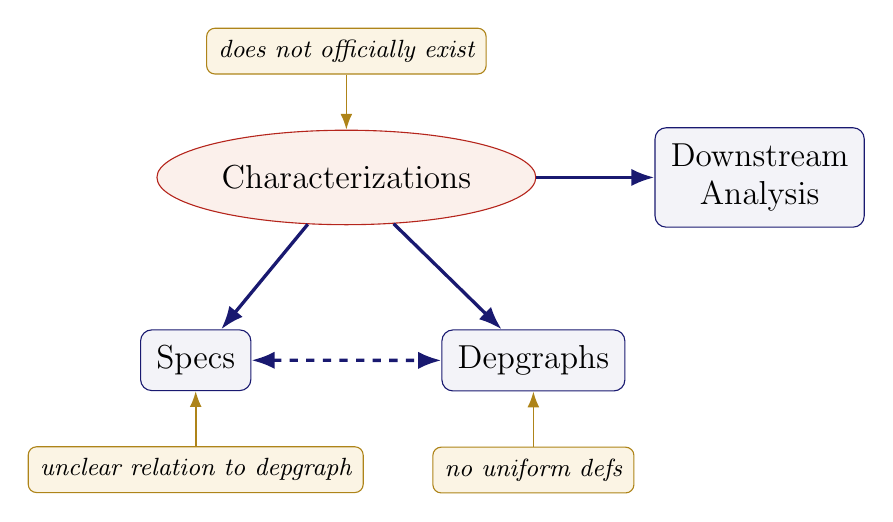
\begin{tikzpicture}[
      >=Latex,
      font = \large,
      box/.style={
        draw = MidnightBlue,
        rounded corners = 4pt,
        fill = MidnightBlue!5,
        align = center,
        inner sep = 2mm,
      },
      annotation/.style={
        draw = Goldenrod!80!black,
        rounded corners = 3pt,
        fill = Goldenrod!12,
        align = center,
        font = \small\itshape,
        inner sep = 1.5mm,
      },
      annotation arrow/.style={
        -Latex,
        semithick,
        Goldenrod!80!black,
      },
    ]
    \node[ellipse, draw = BrickRed,
      fill = BrickRed!5, minimum height = 1.2cm] (c)
      {Characterizations};
    \node[box, below left = 1.5cm and -0.5cm of c] (s) {Specs};
    \node[box, below right = 1.5cm and -0.5cm of c] (g) {Depgraphs};
    \node[box, right = 1.5cm of c] (a) {Downstream\\Analysis};
    \node[annotation, above = 7mm of c] (c-note)
      {does not officially exist};
    \node[annotation, below = 7mm of s] (s-note)
      {unclear relation to depgraph};
    \node[annotation, below = 7mm of g] (g-note)
      {no uniform defs};
    \draw[-Latex, very thick, MidnightBlue] (c) -- (s);
    \draw[-Latex, very thick, MidnightBlue] (c) -- (g);
    \draw[-Latex, very thick, MidnightBlue] (c) -- (a);
    \draw[-Latex, <->, very thick, MidnightBlue, dashed] (s) -- (g);
    \draw[annotation arrow] (c-note) -- (c);
    \draw[annotation arrow] (s-note) -- (s);
    \draw[annotation arrow] (g-note) -- (g);
  \end{tikzpicture}
\end{document}
